\documentclass{article}

\usepackage{a4wide}
\usepackage[utf8]{inputenc}
\usepackage[T1]{fontenc}
\usepackage[french]{babel}
\usepackage[babel=true]{csquotes} % guillemets français
\usepackage{graphicx}
\graphicspath{{Images/}}
\usepackage{color}
\usepackage{hyperref}
\hypersetup{colorlinks,linkcolor=,urlcolor=blue}

\usepackage{amsmath}
\usepackage{amssymb}


\title{Balles en mouvement}
\author{Fabien HOARAU, L3 informatique}
\date{\today}

\begin{document}

\maketitle % pour écrire le titre

%% Le résumé:
\begin{abstract}
Ce rapport a pour but de présenter l'exercices balles en mouvement le tout réalisé en Java.
Je parlerais des différentes méthodes utilisé ainsi que les 	difficulté rencontrées.
\end{abstract}

\section{Introduction}
	\label{section:intro} % pour faire référence à la section 			ailleurs (\ref{...} voir plus bas)
J'ai choisi de développer le programme sous Java car j'ai plus de 	familiarité au niveau des librairies graphique par rapport à 	Python.
Le projet se compose de plusieurs classes toutes aussi 	importantes les unes des autres:

\begin{itemize}
	\item Balle.java
	\item Ecran.java
	\item Fenetre.java
	\item Main.java
	\item Panneau.java
	\item Timer.java
	\item UI.java
\end{itemize}

\vspace{5mm}

Aperçu final de l'application:

\begin{center}
  	\includegraphics[scale=0.6]{apercu.png}
\end{center}

\vspace{5mm}

\section{Développement}
	\subsection{Présentation: la classe balle}
La classe balle représente une grande partie de l'application, 	sans elle aucune balle ne sera présente. Ici la balle est représentée 	par des coordonnées \textit{posX} et \textit{posY} et sa taille avec \textit{radius}.  
\newline

Chaque balles créées sont générées avec des coordonnées aléatoire à l'aide de la fonction \textit{Math.random}
Pour les coordonnées aléatoires, la taille de la balle et de la fenêtre sont prises en comptes. 
\newline

Une balle possède également une couleur elle-même générée aléatoirement.
Pour la gestion de la génération de couleur aléatoire, j'ai utilisé la librairie \textit{java.util.Random;} qui va générer une valeur aléatoire comprise dans un intervalle donnée, ici on fera correspondre ces valeur au code RGB, soit de 0 à 255.
\newline
J'ai ensuite initié 3 variables \textit{redValue},\textit{greenValue} et \textit{blueValue} qui génèrent une valeur entre 0 et 255. Je récupère ensuite ces valeurs pour les appeler lors de l'initiation d'un objet \textit{Color}.
\newline 

\begin{center}
	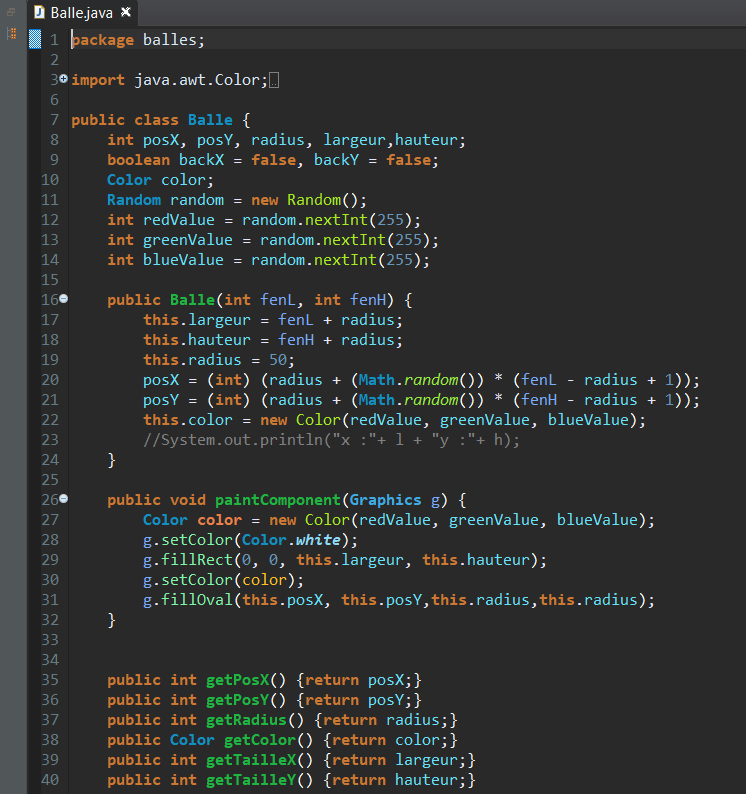
\includegraphics[scale=0.5]{Balle.png}
\end{center}

\begin{center}
  	\textsl{Aperçu de la classe Balle, qui gère la structure d'une balle.}
\end{center}

\newpage
	\subsection{La classe fenêtre}
La classe fenêtre s'occupe de placer les différents éléments (boutons, score, couleur de fond,...). 

\begin{verbatim}
	public Fenetre() {
		this.setTitle("Balles en mouvement");
	    this.setSize(800, 800);
	    this.setResizable(false);
	    this.setDefaultCloseOperation(JFrame.EXIT_ON_CLOSE);
	    this.setLocationRelativeTo(null);
	    //this.setContentPane(panneau);
	    this.setVisible(true);
	    ecran.setBackground(Color.white);
	    add(ecran);
	    add(boutons, BorderLayout.SOUTH);
	    add(textes, BorderLayout.NORTH);
	    boutons.setLayout(new FlowLayout());
	    boutons.add(start);
	    boutons.add(plus);
	    boutons.add(moins);
	    boutons.add(rPlus);
	    boutons.add(rMoins);
	   	//.....
	}	   
\end{verbatim}

On peut remarquer que j'ai mis volontairement l'interdiction du redimensionnement de la fenêtre car si on agrandit la fenêtre les balles générées avant agrandissement de la fenêtre resterons dans la zone 800,800 (taille de la fenêtre de départ). 
\newline
Mais si on agrandit la fenêtre et qu'on ajoute une ou plusieurs balles, ces dernières vont se déplacer dans tout l'espace disponible jusqu'à atteindre un bord ou bien une autre balle.
\newline

\subsection{Le mouvement et la collision(bordures et balles}

\begin{center}
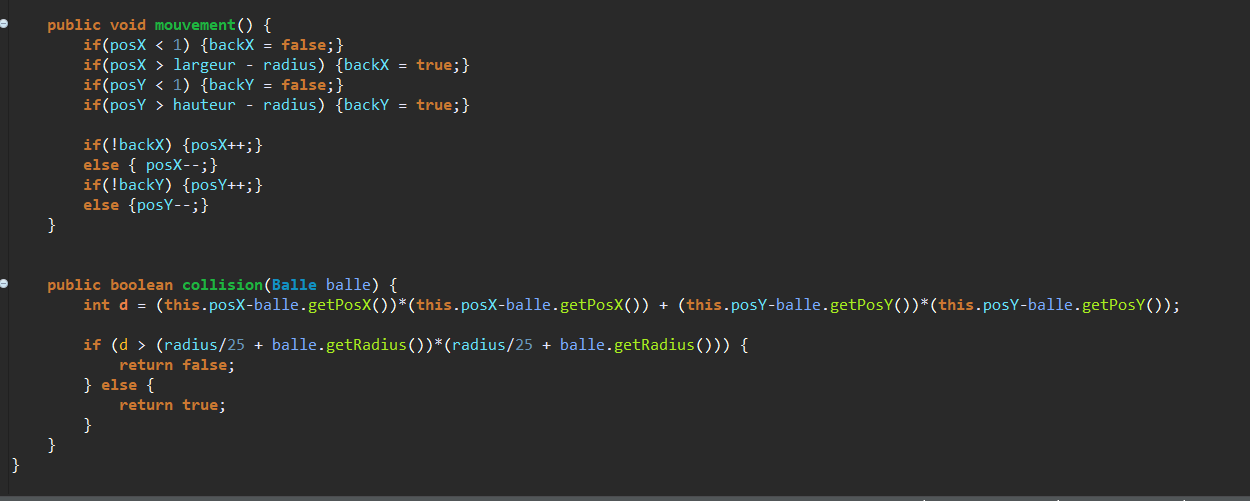
\includegraphics[scale=0.5]{Mouvement_Collision.png}
\end{center}

\begin{center}
\textsl{Gestion du mouvement d'une balle et de la collision avec une autre balle.}
\end{center}

\textbf{Mouvement}: Le code du mouvement est inspiré de la 	méthode du site \href{https://openclassrooms.com/fr/courses/26832-apprenez-a-programmer-en-java/23193-le-fil-rouge-une-animation}{OpenClassroom} sur l'exercice du fil rouge dans le cours sur le 	développement en Java. 
Le code gère également la collision avec les bordures de la fenêtre. 
Les booléens \textit{BackX} et \textit{BackY} permettent de tester si l'on recule ou non sur l'axe x et y.

\vspace{5mm}

\textbf{Collision}: Pour la collision il s'agit également d'un code provenant d'OpenClassroom depuis le cours sur la \href{https://openclassrooms.com/fr/courses/1374826-theorie-des-collisions/1374988-formes-simples}{Théorie des collisions}.
\newline
Le principe: un cercle possède un centre x,y et un rayon. Pour savoir si il y a une collision on teste si le centre x,y se trouve dans le cercle. Pour cela, on calcule la distance du point x,y au centre du cercle à l'aide de Pythagore : \textit{d = sqrt((x-C.x)*(x-C.x) + (y-C.y)*(y-C.y))}
	
\subsection{La classe Timer}
La classe \textit{Timer} est particulière puisque cette classe gère également le score, lorsqu'on fait appel à \textit{setScore()} on incrémente simplement.(\textit{On fait appelle à setScore() lorsqu'il y a une collision voir le \textit{public void run()} dans la classe panneau}. 
\begin{verbatim}
public class Timer extends Thread {
    int timer = 0;
    int score = 0;
    boolean state = false;

    public int getTimer() {return timer;}
    public void setTimer(int timer) {this.timer = timer;}
	
    public int getScore() {return score;}
    public void setScore() {score++;}
    
    public void setEtat(boolean etat) {state = etat;}
    boolean state = false;
    public void run() {
        while(true) {
        if(state) {
            try {
                timer++;
                sleep(1000);
            } catch(InterruptedException e) 
            // TODO Auto-generated catch block
            {e.printStackTrace();}
        } else {
            try {
                sleep(0);
            } catch(InterruptedException e)
            {e.printStackTrace();}
            }
        }
    }
}
\end{verbatim}	

\newpage
\subsection{La classe UI}
La classe UI gère simplement le fait d'afficher le score et le timer dans la fenêtre utilisateur. La classe hérite de JLabel, on peut donc manipuler l'affichage dans la fenêtre grâce aux méthodes :
\begin{itemize}
	\item \textbf{setFont()} : pour définir une police, son caractère et sa taille
	\item \textbf{setText()} : pour pouvoir afficher le score et le temps en récupérant la valeur courante de chacune de ces variables grâce à \textit{timer.getScore()} et \textit{timer.getTimer()}
	\item \textbf{setForeground()} : pour définir une couleur
	\item \textbf{setHorizontalAlignment()} : pour l'alignement horizontal
\end{itemize}

\vspace{5mm}

 La déclaration de la variable \textit{timer} du type \textbf{Timer} permet de manipuler les variables score et timer de la classe Timer

\begin{verbatim}
public class UI extends JLabel {
    Timer time;
    
    public UI(Timer time) {
	    this.time = time;
	    this.setFont(new Font("Emulogic", Font.BOLD, 12));
	    this.setText("Score : " + time.getScore() + "Temps : " + time.getTimer());
	    this.setForeground(Color.blue);
	    this.setHorizontalAlignment(CENTER);
    }
	
    public void paintComponent(Graphics g) {
        this.setText("Score : " + time.getScore() + " Temps : " + time.getTimer());
        super.paintComponent(g);
        repaint();
    }
}
\end{verbatim}


\subsection{Points délicats/intéressants}
\subsubsection{Points délicats : le mouvement} Le code du mouvement d'OpenClassroom ne fonctionnait que pour une seule balle, il fallait l'adapter pour plusieurs balles, pour cela j'ai utilisé les\textit{ArrayList}.

\begin{center}
	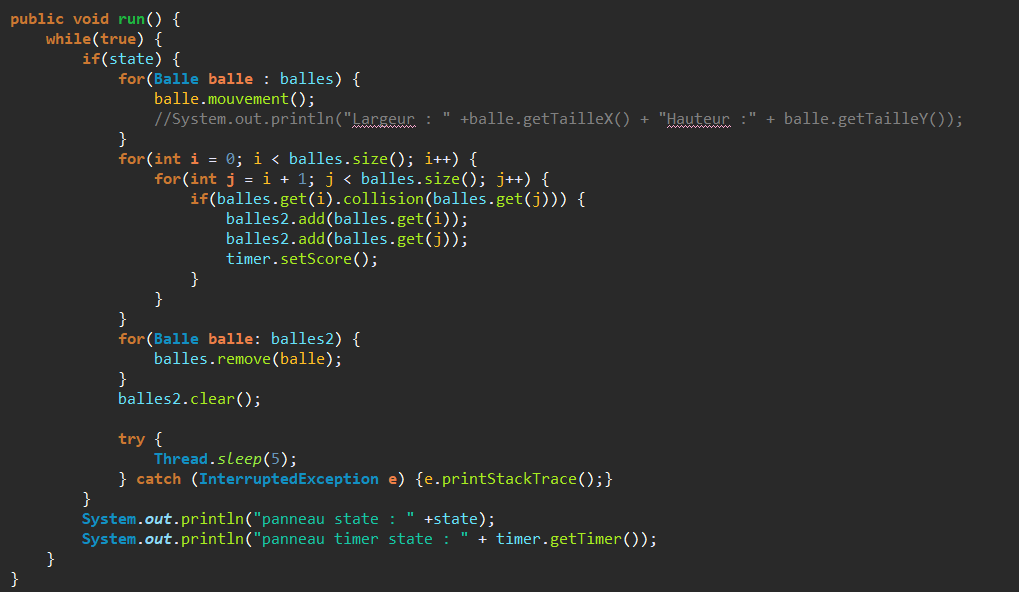
\includegraphics[scale=0.5]{runMouvement.png}
\end{center}
\textit{L'ensemble des explications données ci-dessous dépendra de la variable booléenne \textbf{state}, si elle est à \textbf{true} on exécute tout.}
	
	
\textbf{Principe}: On possède deux listes : 
\newline
	
La première liste : \begin{verbatim}ArrayList<Balle> Balles = new ArrayList<Balle>();\end{verbatim} 
La deuxième liste : \begin{verbatim}ArrayList<Balle> Balles2 = 	new ArrayList<Balle>();\end{verbatim} 
La première liste va s'occuper de lister les balles qu'on a ajoutées. En parcourant la liste on vérifie si il y a au moins une balle, si c'est le cas on lance le mouvement grâce à la fonction \textit{mouvement()}.

\begin{verbatim}
for(Balle balle : balles){
   balle.mouvement();
}
\end{verbatim}	

La deuxième liste gère les balles qui sont entrées en collisions, si c'est le cas on ajoute ces balles dans cette seconde liste, puis en parcourant la liste on supprime ces balles.


\subsubsection{Points délicats : le timer}
Pour le timer c'était un problème mineur au niveau d'une variable:
Voici le code lorsqu'il y avait un problème:
	
\begin{verbatim}
public class Timer extends Thread {
    //...
    boolean state = false;
    public void run() {
        while(true) {
        if(state) {
            try {
                timer++;
                sleep(1000);
            } catch(InterruptedException e) 
            // TODO Auto-generated catch block
            {e.printStackTrace();}
            }
        }
    }
}			   
\end{verbatim}		

Le problème se trouvait au niveau du \textit{public void run()}, en effet, lorsque je lançais le programme, et que j'appuyais sur le bouton start, le timer se lançait normalement (ainsi que le mouvement des balles) et s'arrêtait lorsque j'appuyais de nouveau.
Mais si j'appuyais de nouveau le bouton start, le mouvement se lançait bien mais pas le timer.
\newline
Pour résoudre ce problème j'ai simplement rajouté un \textit{else} pour vérifier le cas où la variable \textit{state} est à \textit{false}

\newpage
\begin{verbatim}
public class Timer extends Thread {
    //...
    boolean state = false;
    public void run() {
        while(true) {
        if(state) {
            try {
                timer++;
                sleep(1000);
            } catch(InterruptedException e) 
            // TODO Auto-generated catch block
            {e.printStackTrace();}
        } else {
            try {
                sleep(0);
            } catch(InterruptedException e)
            {e.printStackTrace();}
            }
        }
    }
}			   
\end{verbatim}	


\subsubsection{Points délicats : la collision}
Un autre point particulier se trouve au niveau de la fonction \textit{collision} de la classe \textit{Balle}.

\begin{center}
	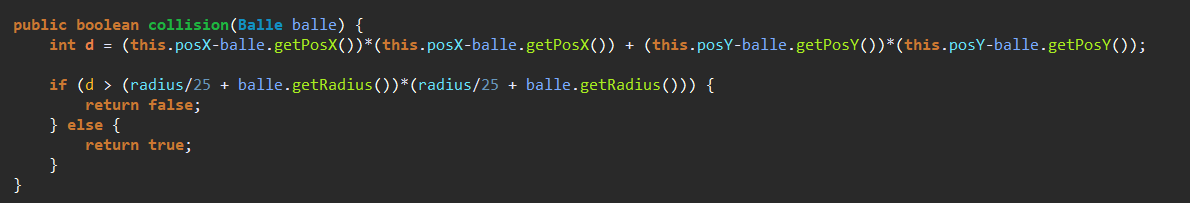
\includegraphics[scale=0.5]{Collision.png}
\end{center}
On peut voir que j'ai divisé le \textit{radius} par 25. Sans cela les collisions allaient s'effectuer de manière "trop proche".
\newline
En divisant le \textit{radius} par une certaine valeur on réduit la taille de la collision pour éviter les collisions trop proches.

\subsubsection{Points intéressants : l'ajout de bouton}
Sur le rendu final on peut voir qu'il y a deux boutons qui ont été rajoutés.

\begin{center}
	
\includegraphics[scale=0.8]{Boutons.png}
\end{center}

\textbf{Que font-ils ?}
Ils ont une simple fonctionnalité : il augmente simplement la taille (\textit{radius}) de 10, des balles présentes, lorsqu'on appuie sur le bouton \textbf{Taille+} et inversement, on diminue sa taille de 10, si on appuie sur \textbf{Taille-}.
\newline

Il y a cependant quelque problèmes mineur qui surviennent : 
\begin{itemize}
	\item si la taille d'une balle est supérieure à une autre balle la collision risque d'être faussée.
	\item si on diminue fortement la taille de la balle, l'utilisateur risque de ne plus voir la balle à l'écran, par contre elle sera toujours en mouvement, suivant l'état du bouton \textbf{start}.
\end{itemize}


\begin{center}
	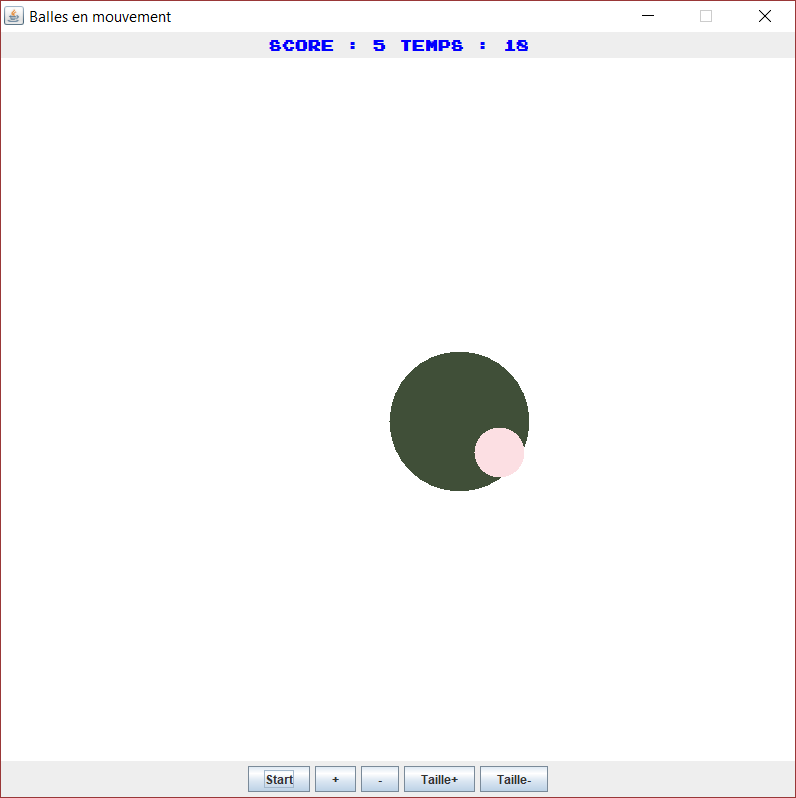
\includegraphics[scale=0.5 ]{ProblemeCollision.png}
\end{center}

\begin{center}
  	\textsl{Problème de collision si les tailles des balles sont différentes}
\end{center}

\section{Conclusion}
Pour conclure ce rapport, ce projet m'a permis d'étendre plus de connaissances sur le langage java ainsi que les différents procédés et moyens utilisés pour pouvoir réaliser cette application. Il y a encore certaines subtilités, comme par exemple la gestion de la taille. En rajoutant ces fonctions j'ai pu m'apercevoir que la collision ne fonctionne pas complètement lorsqu'on change la taille d'une balle. 

%%% La bibliographie:
\nocite{*}

\bibliographystyle{plain}
\bibliography{biblio}




\end{document}
